\chapter{Глава 1}
Что ж, вот и пришло время приступить к новому циклу. На сей раз речь пойдёт о Японии. Автора этих строк всегда интересовал следующий вопрос – почему в 1941 году Страна Восходящего солнца нанесла удар не по скованному чудовищного масштаба противостоянием в Европе Советскому Союзу, а по Соединённым Штатам. Во многих отношениях это кажется нелогичным. Япония совместно с Германией ещё в 1936 году подписала Антикоминтерновский пакт – к слову, документ весьма любопытный, вроде бы как союзный договор, а вроде бы и совершенно нет, но, так или иначе, истинная цель его была прозрачна – противодействие СССР. В 1940 японцы присоединятся к Берлинскому пакту. В 1941 и 1942 году Германия несколько раз совершенно недвусмысленным образом намекала на то, что неплохо бы японцам об этих договорах вспомнить. В июле 1941 года министр иностранных дел Третьего Рейха Иохим фон Риббентроп отослал инструкцию послу в Японии, Отту: «Я прошу Вас продолжать прилагать усилия к тому, чтобы добиться скорейшего участия Японии в войне против России. Используйте все имеющиеся в Вашем распоряжении средства, потому что, чем раньше осуществится это участие в войне, тем лучше. Как и прежде, цель, естественно, должна заключаться в том, чтобы Германия и Япония встретились на Транссибирской железной дороге до наступления зимы».


У Японии и России, причём, что любопытно, как Царской, так и Советской, уже была богатая история противостояния. Русско-Японская война, участие Японии в Интервенции, масса пограничных инцидентов после установления японской власти в Маньчжурии, самый крупный из которых – бои у озера Хасан. Наконец, почти что полноценная война у Халхин-Гола, в которой японцы несут потери как минимум не уступающие потерям вермахта в Польской кампании. 

\begin{figure}[h!tb] 
	\centering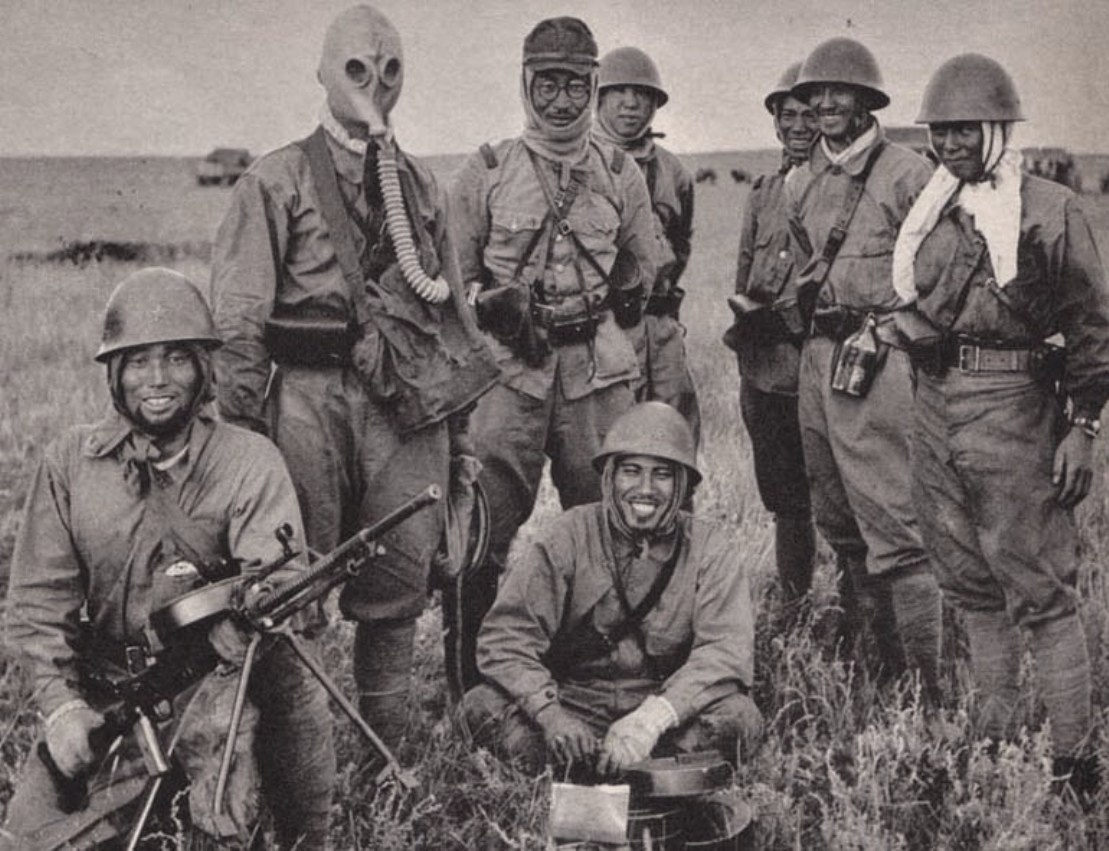
\includegraphics[scale=0.45]{Glava1/ElRqW9KibOM.jpg}
	%	\label{fig:scipion} % Unique label used for referencing the figure in-text\end{document}
	%	%\addcontentsline{toc}{figure}{Figure \ref{fig:placeholder}} % Uncomment to add the figure to the table of contents%----------------------------------------------------------------------------------------
	\caption{Японские солдаты под Халхин-Голом, 1939. Обратите внимание на трофейный ДТ у одного из сидящих}%	CHAPTER 2
\end{figure}

В то же время с США Япония не скрещивала шпаг ни разу. Даже в 1853 году эскадра коммодора Перри “открывая” Страну восходящего солнца стреляла у берегов Эдо(Токио) лишь холостыми. Далее – возможный куш. В случае с ударом по Советскому Союзу им мог стать весь Дальний Восток, а может быть более обширные регионы Сибири. По ряду сведений немцы были готовы отказаться от претензий на все территории, лежащие восточнее 70° восточной долготы. В любом случае, Статья 2. Берлинского пакта гласила: “Германия и Италия признают и уважают руководящее положение Японии в установлении нового порядка в Великой Восточной Азии”. С другой стороны о возможностях территориальных приобретений за счёт США (кроме Филиппинских, Гавайских и ряда более мелких островов) никто и никогда не говорил всерьёз.

Вообще сами японцы очень чётко определяли перспективу высадки экспедиционного корпуса где-нибудь под Сан-Франциско с дальнейшим походом в сторону Скалистых гор как полную утопию. Особенно же ясно это понимали те военно-морские командующие, которые в дальнейшем и вели боевые действия против Штатов. Так, на стадии обсуждения плана атаки на Перл-Харбор, один из ведущих оппонентов этого плана начальник штаба 11-й воздушной армии Ониси Такидзиро сказал дословно следующее: «В любой войне с США Япония не в состоянии поставить противника на колени. Вступить в войну, не имея этой способности, означает, что мы обязаны отыскать возможность короткой войны, что, в свою очередь, диктует нам необходимость в какой-то момент достичь компромисса. По этой причине, высадим мы десант на Филиппинах либо где-нибудь еще, нам следует избегать таких предприятий, как Гавайская операция, — она здорово разозлит Америку». Что уж тут говорить о каких-либо действиях непосредственно на Североамериканском континенте. К слову, спорил Такидзиро с адмиралом Исоруку Ямамото, который чуть ли не меньше всех был склонен недооценивать США и отводил своему собственному флоту примерно 1,5 года достаточно успешного противодействия американцам, а после этого срока считал неизбежным более или менее быстрое и полное, но поражение, если не произойдёт каких-либо глобальных политических перемен.

Отношение японского флота к перспективе войны хорошо иллюстрирует следующий инцидент, имевший место в начале августа 1941. Тогда глава 1-го сектора 1-го управления морского генерального штаба Томийока Садатоши поручил своим подчиненным начать подготовку к войне. Когда капитан 3-го ранга Мийо выразил недовольство — он не уверен в шансах Японии в войне с Америкой, — Томийока вспыхнул от гнева.

— Чушь! — воскликнул он. — Воюют не потому, что кто-то уверен или не уверен! Решение об этом принимает правительство. Что это за флот, если на объявление правительства: «Война!» — мы ответим: «Извините, но у нас нет уверенности, поэтому мы никак не готовились»?!

Или ещё более определённые выражения из меморандума (уже не обсуждения и не фразы, но вполне официального документа), подготовленного командиром флотского департамента аэронавтики Инуэ Сигейоси в 1940: «…Ясно, что при правильной политике в области вооружений для Японии возможно избежать поражения от Америки, и естественно надеяться, что именно так и будет. Но с другой стороны, Японии не победить Америку и не заставить ее капитулировать. В причине здесь нельзя ошибиться… Американские операции против Японии будут те же, что японские против Америки, в том смысле, что Япония находится на огромном расстоянии от Соединенных Штатов; но в других отношениях они очень отличаются друг от друга, потому что Америка сможет: 1) оккупировать всю территорию Японии; 2) захватить столицу Японии; 3) в войне стереть с лица земли японские войска».

Итак, у ведущих руководителей флота наличествует точное и ясное понимание того, что Япония неспособна силовыми действиями заставить Соединённые Штаты признать своё поражение, тем более, полностью их разгромить и уничтожить как значимую державу. Максимум возможного – временное выведение из строя американского флота (и то не всего, а только Тихоокеанского – Атлантика для японского Объединённого флота совершенно недосягаема), достижение локального господства на море на 1-1,5 года и… Что потом? Чем Япония рискует очевидно – а вот что она надеется достигнуть, так сказать, по варианту максимум?

Или же дело не в куше, а в угрозе? Япония вполне понимает, что по всем параметрам (кроме, быть может, достаточно неопределённых моральных) она в целом и её вооружённые силы в частности уступают США. В некоторых аспектах – на порядок. Слабейший (и знающий это) атакует сильнейшего. Как правило, такие действия диктуются стремлением упредить истинные или мнимые действия противника. Сейчас нам совершенно ясно и достоверно известно, что у Соединённых Штатов не существовало агрессивных планов в отношении Японской империи. Да, у ВМС США был так называемый Оранжевый план на случай войны с японцами, он регулярно обновлялся, но это лишь часть обычного военного планирования, а характер плана, хотя и наступательный, исходил из того, что военные действия будут начаты Японией. Никаких, даже словесных проектов высадки на Хонсю или какой-либо другой остров Японского архипелага, или чего-то в подобном роде в Америке до декабря 1941 года не было. Положим, японская разведка могла не знать об этом, но политическая ситуация в США, массовое нежелание втягиваться в очередную мировую войну в народе, обеспокоенность ситуацией в Европе у элит как будто не давала оснований для предположений о готовящейся агрессии. Тогда чего японцы боялись? Почему с начала 1941 года о столкновении с Америкой на флоте начинают говорить как об очень опасном, нежелательном, но, по-видимому, неизбежном?

К слову, здесь уместно напомнить, что с 1937 года Япония уже вовлечена в крупномасштабную войну в Китае, которая по совокупности жертв на начало 1941 года – до вторжения вермахта в СССР, значительно превосходит боевые действия в Европе. И, тем не менее, страна буквально бросается в ещё одну – и куда более тяжёлую. Причём нельзя сказать, чтобы в 1940 или 1941 японцы достигли в Китае столь значимых успехов, чтобы можно было, даже и ошибочно, списать этот ТВД со счетов. Общеизвестен и тот факт, что, несмотря на мир с СССР численность Квантунской армии неуклонно росла до 1945 года, т.е. неверно утверждать, что договор о нейтралитете, подписанный в апреле 1941 с Советским Союзом, позволил правительству и военному командованию Японии решительно перебросить свои резервы на другие операционные направления. Но тогда с ещё большей силой перед нами встаёт вопрос – почему? Почему был сделан выбор в пользу войны с Соединёнными Штатами? В уме всплывают какие-то достаточно неопределённые вещи в том духе, что США препятствовали японской экспансии – но как именно, в чём это выражалось, а главное – почему в итоге привело к Перл-Харбору? 

\begin{figure}[h!tb] 
	\centering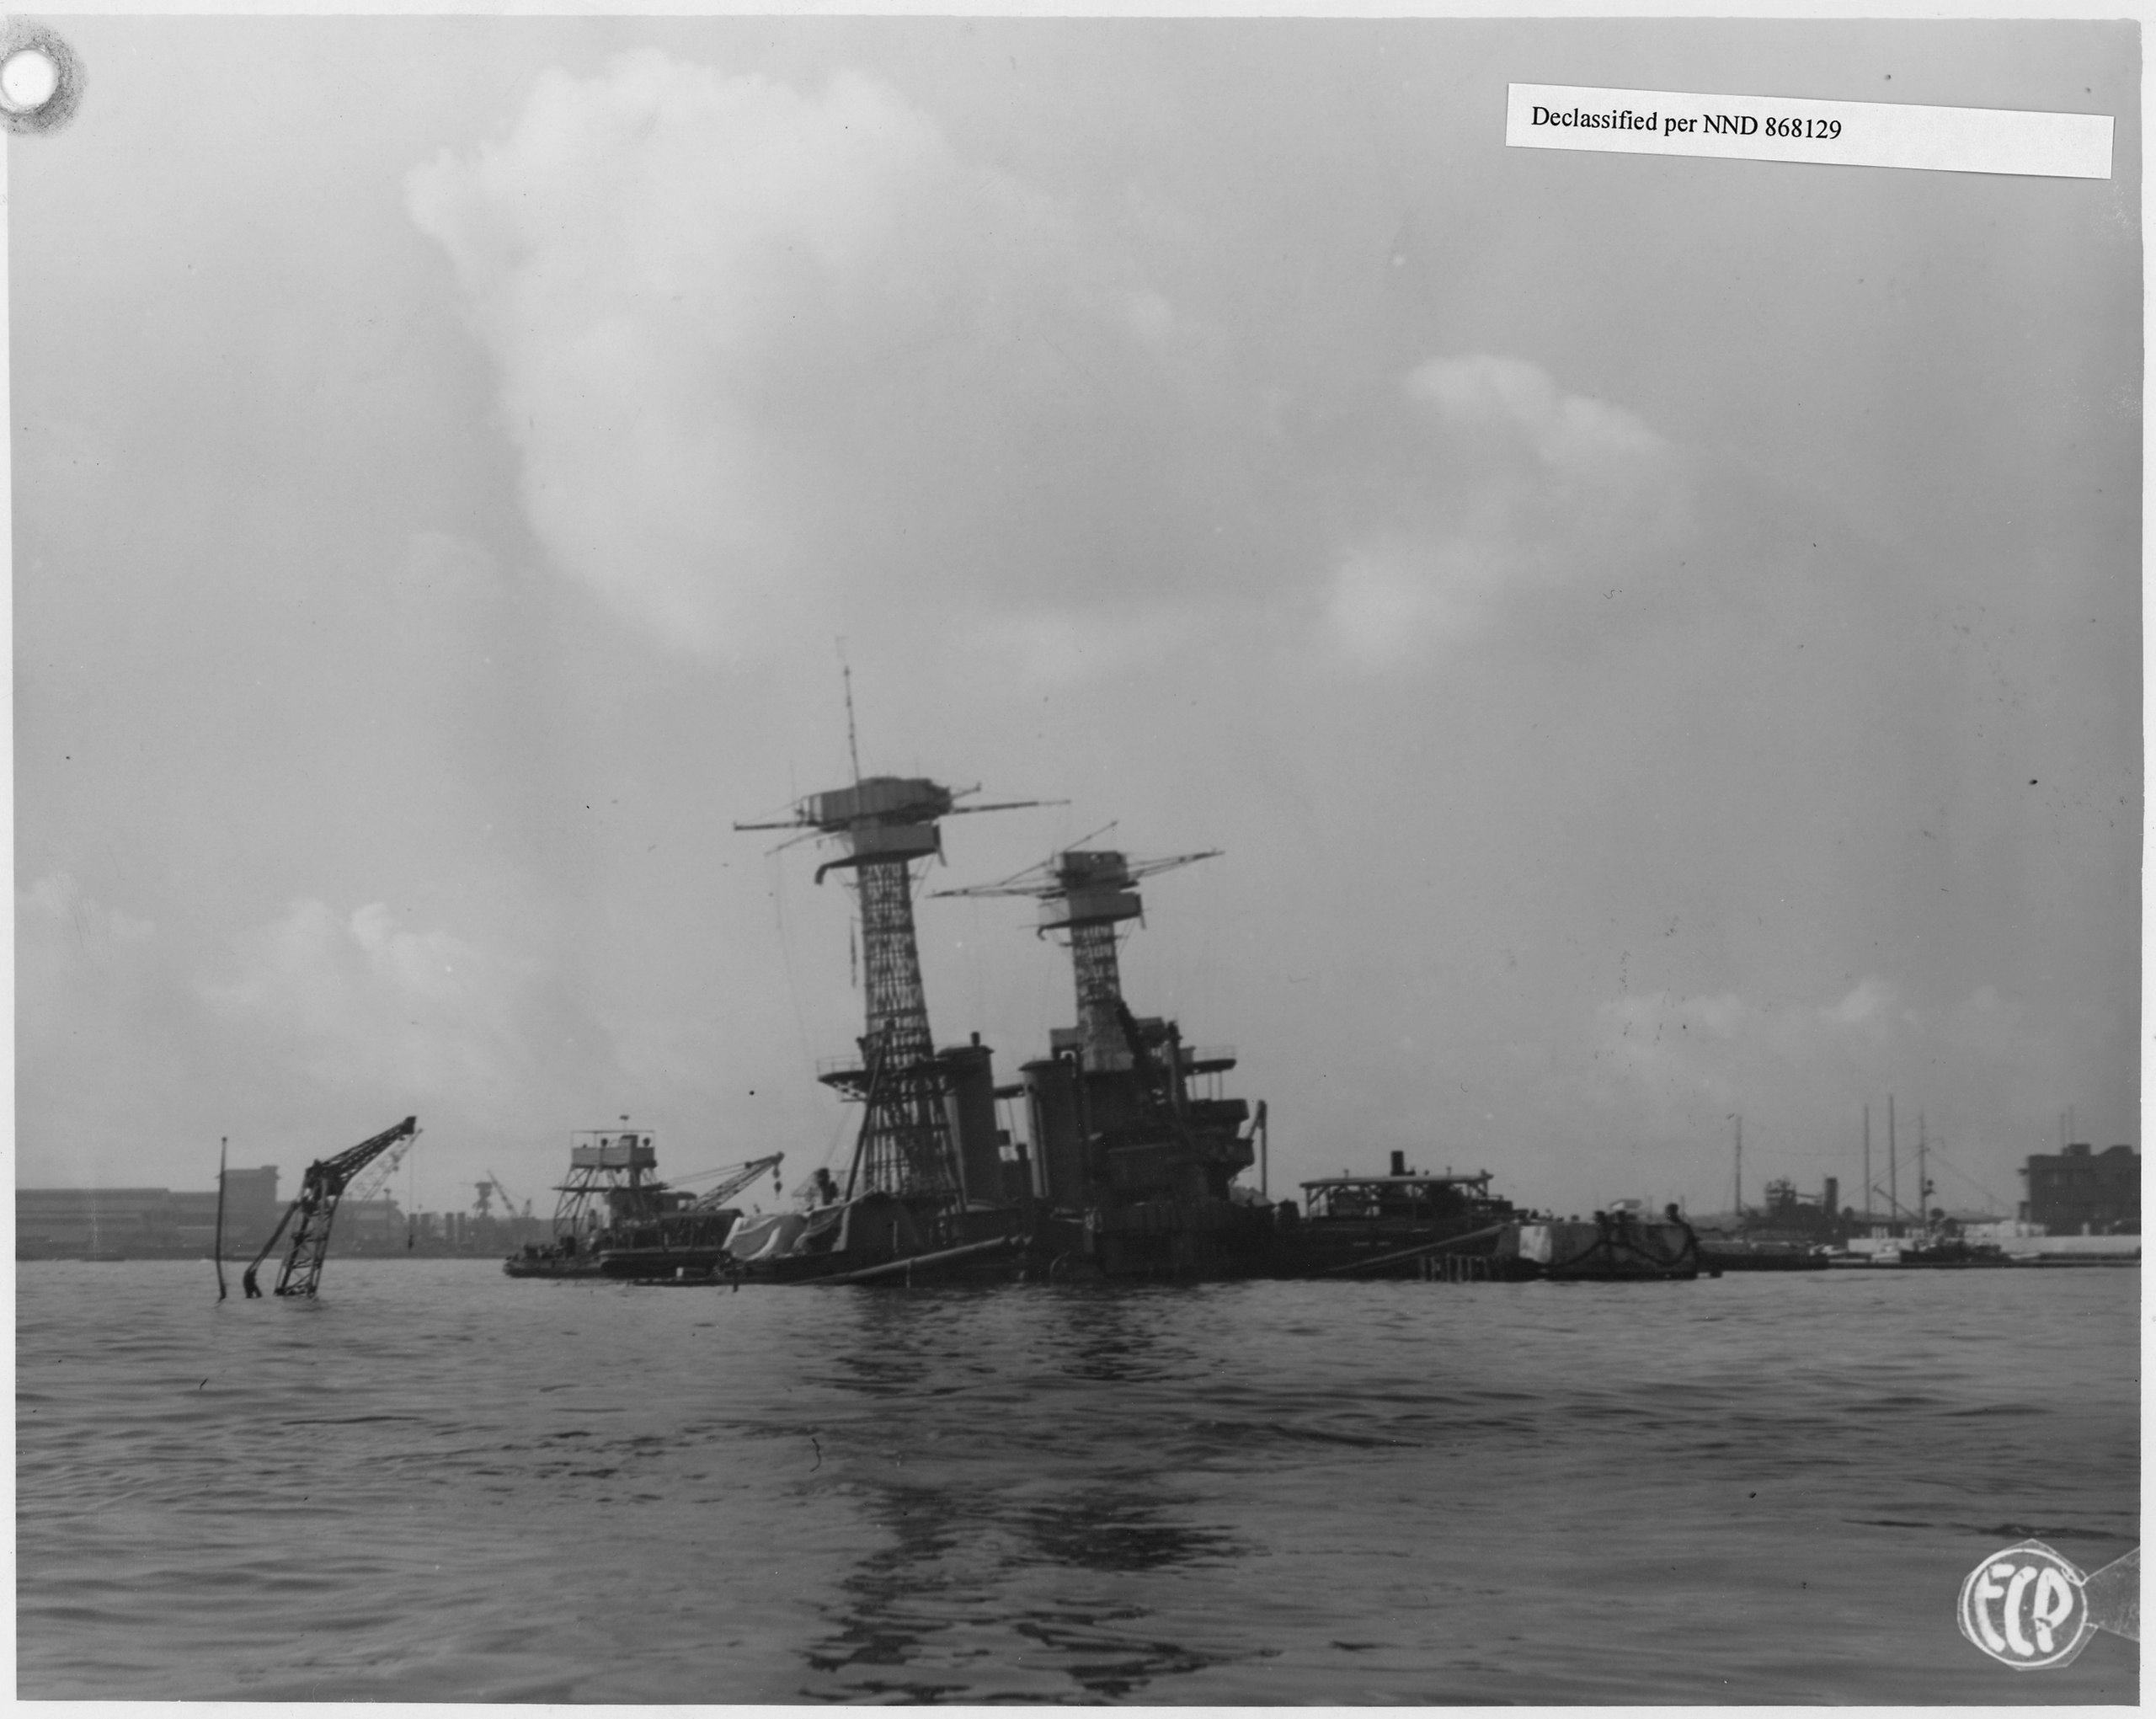
\includegraphics[scale=0.5]{Glava1/UWUiFP19AEM.jpg}
	%	\label{fig:scipion} % Unique label used for referencing the figure in-text\end{document}
	%	%\addcontentsline{toc}{figure}{Figure \ref{fig:placeholder}} % Uncomment to add the figure to the table of contents%----------------------------------------------------------------------------------------
	\caption{Затопленный в гавани Перл-Харбора линкор Калифорния, 1941}%	CHAPTER 2
\end{figure}


Для начала разберёмся с принципиальным вопросом – почему Японии вообще была нужна (подчеркну это – действительно, на самом деле необходима) экспансия. Поможет нам здесь статистика. За отправную точку возьмём примерно 1600 год – в это время прошло два года с момента смерти первого объединителя Японии – Тоётоми Хидэёси. Финальный раунд борьбы за власть между его сыном Хидэёри и влиятельным соратником/союзником Токугава Иэясу ещё впереди, но в основном период междоусобных войн можно считать оконченным. Сражаются уже за власть над страной, но никак не за то, чтобы вновь расколотить её на множество мелких осколков. Существуют различные оценки численности населения Японии в это время, разбросанные от 10 до 20 миллионов человек. Наиболее вероятная цифра – 15-16 миллионов. Много это, или мало? Ну, к примеру, это в три раза больше, чем население в тот же период времени Русского Царства… Но дальше следует продолжительный период внешнего и внутреннего мира. Перепись населения 1721 даёт 26 065 425 человек. И это уже совершенно определённо много. Число жителей Страны Восходящего солнца превосходит самое густонаселённое государство Европы того времени – Францию – там в 1730 насчитывается 23 800 000. За 121 год японцев стало больше примерно на 10 миллионов. Теперь же сделаем ещё один скачок длинной чуть более чем в столетие. В 1846 году перепись показала… 26 907 600 человек. Иными словами прирост меньше миллиона. При этом – по-прежнему мир, покой, нельзя сказать, что какая-то сила проредила молодую поросль нации мечом. Тогда в чём же дело?

Кто-то из читателей может предположить – дело в эпидемиях. Могучие удары болезней, столь чувствительные в те годы, забрали массу жизней и не дали численности населения возрастать так же быстро, как прежде. Но и это не так – мы не располагаем информацией о катастрофических эпидемиях в Стране Восходящего солнца в 1721-1846. Зато у нас предостаточно сведений о чередующихся периодах массового голода. Голод Кехо, начавшийся в 1732, уменьшил население страны на 850 тысяч к 1750 году. Следующие 30 лет население Японии оставалось примерно одинаковым. Великий голод Тэммэй 1783—1787 годов уменьшил население Японии более чем на 1 миллион человек. После этого до 1830-х годов население Японии росло и снова достигло цифры в примерно 27 миллионов человек. Великий голод Тэмпо 1833—1836 годов снова сократил население Японии на целый миллион, чтобы оно вновь восстановилось 10 лет спустя.

Эти цифры говорят об одном – Япония достигла естественного предела. Без крупных регулярных торговых связей, в рамках традиционного хозяйства без технических новшеств земля не могла прокормить большее количество людей, чем плюс-минус малость 27 миллионов. К моменту силового вывода империи из её самоизоляции в 1853 эта цифра была превзойдена очень незначительно. Далее внешнеэкономические связи стали лавинообразно нарастать – и с ними приходить первые ростки новых технологий. Но переломом, естественно, стала Реставрация Мэйдзи. После обретения полноты власти императором-реформатором история Японии пустилась буквально вскачь – и это в полной мере касается и населения. На 1898 год японцев уже 46 миллионов. А далее масштабы роста только увеличиваются. В 1910 – уже 51 миллион. В 1925 – почти 60 миллионов. И тогда же пика достигает рождаемость. После 1930 она медленно начнёт идти на спад, но, во-первых, этого никто не мог тогда толком просчитать как долгосрочную тенденцию, а во-вторых, всё равно она ещё многие годы будет оставаться весьма значительной – настолько, что даже с учётом потерь войны обеспечит Японии к 1966 100 миллионов. Если бы Второй Мировой не было, то следовало бы с учётом непрямых демографических потерь накинуть ещё миллионов так 10-15. В реальности к концу XX века на Японских островах жило 126 с лишним миллионов человек. У тех, кто смотрел в будущее своей страны в 1920-х, кто делал прогнозы, были все основания предполагать 200 миллионов. Для маленькой и гористой Японии это бешено много. Плюс, стоит напомнить, что стигмат и родовая травма Страны Восходящего солнца это вулканизм, землетрясения и цунами. При подобной скученности каждое из них становилось бы неизбежно катастрофой со многими тысячами жертв. Даже и в современной Японии, которая очень далеко шагнула вперёд по части изобретения технологии защиты и предупреждения населения, периодически не удаётся выйти сухими из воды. Жертвами цунами 2011 года стали почти 20 000 человек. Опять таки, в 1920-х и 1930-х не могли рассчитывать на все современные средства защиты, но предполагать сами землетрясения очень даже могли.

В общем, Япония и японцы нуждались не в чём ином, как в жизненном пространстве И это не фигура речи. К слову, занятно будет сравнить ситуацию в Стране Восходящего солнца и в Германии, где один несостоявшийся художник очень много говорил и писал о походе на Восток за землёй – и, в том числе на этом, пришёл в 1933 году к власти. В Германии тогда было 66 миллионов жителей. В Японии на тот же год – примерно столько же. Но в 1940 в Рейхе (без учёта Австрии и Судет) – 69 миллионов, а в Японии уже 73 – и перспективы увеличения разрыва. При этом Германия – это по большей части равнина, ни о каких извержениях и цунами там слыхом не слыхивали. Но и это не всё. От населения мы переходим к ресурсам и сырью. О, сколько жалоб можно найти в немецких мемуарах относительно топливного вопроса. Ох уж это дорогое и трудоёмкое в изготовлении искусственное горючее! Да, всё так, чистая правда. Да, Германия не особенно богата сырьём… в сравнении с СССР, США, или колониальными империями! Но, к примеру, такими стратегически важными ресурсами, как уголь и руда, она обеспечена в достатке. Бассейны Рура и Силезии не зря стали надёжной основой как немецкой металлургии, так и военной промышленности.

Япония же – геологический феномен. Обыкновенно на территориях, прилегающих к крупным разломам и точкам соприкосновения тектонических плит интересного и полезного довольно много. Хоть бы даже кимберлитовые трубки с алмазами. Но в Японии нет ни черта! Вплоть до настоящего времени основу рудной промышленности страны составляет добыча малоинтересной серы. Руды ценных металлов, уголь, нефть, газ – всё это не про Страну Восходящего солнца. В подконтрольной Корее ситуация была несколько лучше – но не настолько, чтобы это радикально меняло дело. Глобально для Японии вырисовывалась следующая перспектива: за счёт собственного сельского хозяйства прокормить стремительно растущее население невозможно – только внешняя торговля, только импорт. За счёт чего при этом формировать национальный доход? Развитие промышленности позволило не только заполнить в основном внутренний рынок, но и начать активно экспортировать товары, но… Очень скоро собственного сырья стало нахватать для развёртывания и расширения производства. Да, ресурсы тоже можно покупать, но тогда их стоимость придётся включить в конечную цену экспортируемых изделий – и в конкурентной борьбе на мировом рынке они начнут проигрывать. Итог – при первом же крупном экономическом кризисе, сокращающем спрос, обвал всей экономической системы и полный крах, причём с очень сомнительными перспективами всплыть на поверхность. Единственная альтернатива – создание устойчиво своих рынков сбыта.

Т.е. всё то же решение – экспансия, приобретение колоний! Страна Восходящего солнца была вольна выбирать способ и направление достижения этой цели, но сам этот рывок вовне был практически неизбежным, если только руководство страны не готово было сознательно пойти на политику жесточайшего самоограничения – фактически – добровольную кастрацию промышленности и драконовские меры в социальной сфере. Всерьёз подобного никто в Японии не рассматривал.

Кто-то спросит: а как же современная Япония? Почему с ней ничего подобного не приключилось, хотя у неё нет ни колоний, да и сырья в недрах не прибавилось? Ответ кроется в том, что после 1945 года долгое время будущим страны распоряжались на столько японцы, сколько американцы, которые в своих интересах и на своих условиях, при которых японцы мало где напрямую оказывались конкурентами США, включили страну Микадо в мировую систему хозяйствования и разделения труда. Свою роль в своё время сыграла и дешевизна рабочей силы. Но весьма примечательно следующее – у знаменитого японского экономического чуда датой начала считается середина 1950-х годов, а конец известен совершенно точно – это нефтяной кризис 1973. Япония была и остаётся одним из основных потребителей нефти Ближнего Востока. И совершенно не случайно, что крупнейший в истории супертанкер Knock Nevis был спроектирован в Японии и построен в Йокосуке. 

\begin{figure}[h!tb] 
	\centering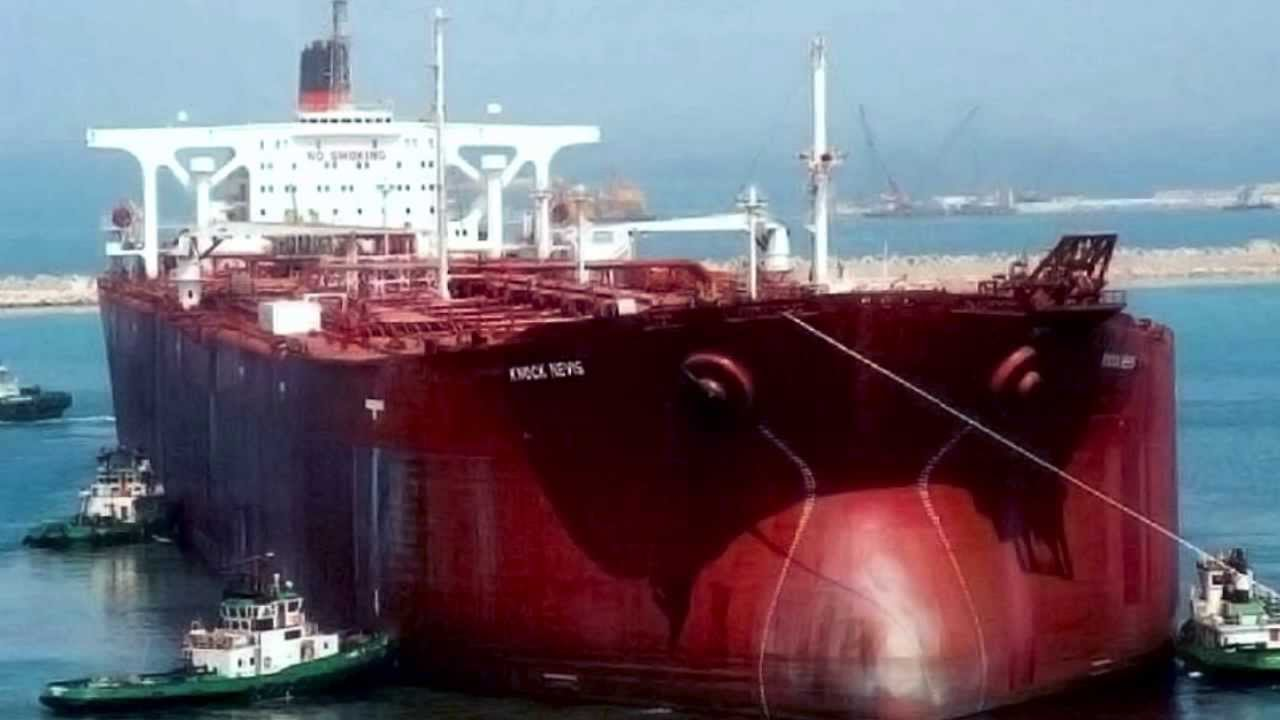
\includegraphics[scale=0.4]{Glava1/L-8_vonVRG0.jpg}
	%	\label{fig:scipion} % Unique label used for referencing the figure in-text\end{document}
	%	%\addcontentsline{toc}{figure}{Figure \ref{fig:placeholder}} % Uncomment to add the figure to the table of contents%----------------------------------------------------------------------------------------
	\caption{Knock Nevis}%	CHAPTER 2
\end{figure}

И уже в наше время, когда мы слышим о напряжённости в японо-китайских отношениях, о том, что Японии не нравится китайская активность на морях и их насыпные острова, то в первую очередь это связано с тем, что Китай берёт под надёжный контроль пути поставки в Страну Восходящего солнца топлива.
Японцы осознают свою зависимость очень четко – и пытаются с ней бороться, но сделать могут не так много. Одним из способов в своё время стало форсированное развитие ядерной энергетики. Самые мощные по суммарной генерации энергоблоков АЭС в истории были построены в Японии. До катастрофы на Фукусиме 2011 года 30\% произведённой в Японии энергии приходилось на долю мирного атома. При этом, хотя вообще автор сих строк является убеждённым сторонником ядерной энергетики, в случае с такой геологической зоной, на которой находятся Японские острова, это действительно очень и очень опасная лотерея. По-настоящему надёжной защиты от землетрясений и, особенно, цунами просто нет. Весь вопрос в критичности и масштабе происходящего. Фукусимская АЭС могла выстоять при волне в 10 метров. Но вот 15 оказались уже чересчур. 


\begin{figure}[h!tb] 
	\centering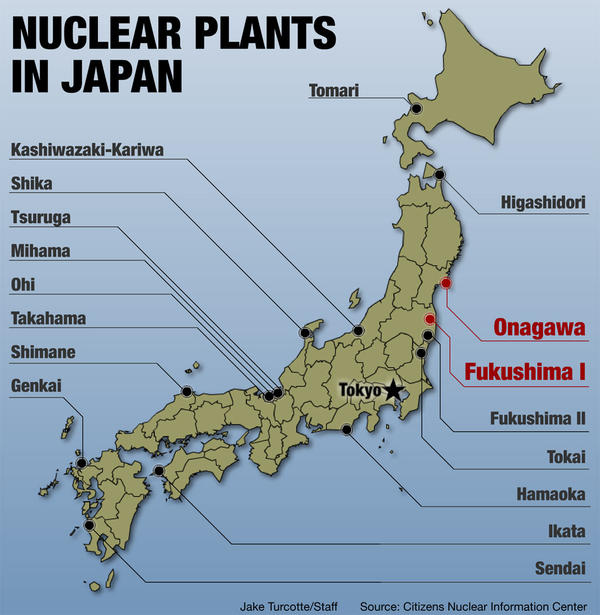
\includegraphics[scale=0.5]{Glava1/RyxsRW6tQYs.jpg}
	%	\label{fig:scipion} % Unique label used for referencing the figure in-text\end{document}
	%	%\addcontentsline{toc}{figure}{Figure \ref{fig:placeholder}} % Uncomment to add the figure to the table of contents%----------------------------------------------------------------------------------------
	\caption{Схема расположения АЭС в Японии}%	CHAPTER 2
\end{figure}

Очень показательно и то, что было после аварии. В 2012 году в стране были остановлены все действующие станции. За исключением двух блоков ситуация оставалась той же и в 2013. А вот потом станции снова начали запускать, параллельно резко пригасив всю фукусимскую тему в СМИ и уменьшив показательно зону отчуждения с 40 до 10 километров. Дошло до события для Японии беспрецедентного – правительство страны нарушило публично данное обещание относительно сокращения и закрытия атомных станций. А причина – в экономике. Обнаружилось, что без них страна просто не способна обойтись. Придётся или радикально наращивать объёмы ввозимого топлива, или устанавливать квоты и лимиты энергопотребления в промышленности (граждане и так приучены к экономии) – и тем самым откровенно её душить. Одним словом, даже в XXI веке кое-что от прежних проблем осталось.
Нынешняя Япония, так сказать, насильственно мирная страна – но для Японии 1920-х, страны с мощной военной кастой, страны-победительницы (последовательно три победы в Японо-китайской, Русско-японской и Первой мировой) мысль о расширении пределов и установлении своей зоны контроля вооружённой рукой была до такой степени естественной, что можно даже сказать – почти неизбежной. 

\begin{figure}[h!tb] 
	\centering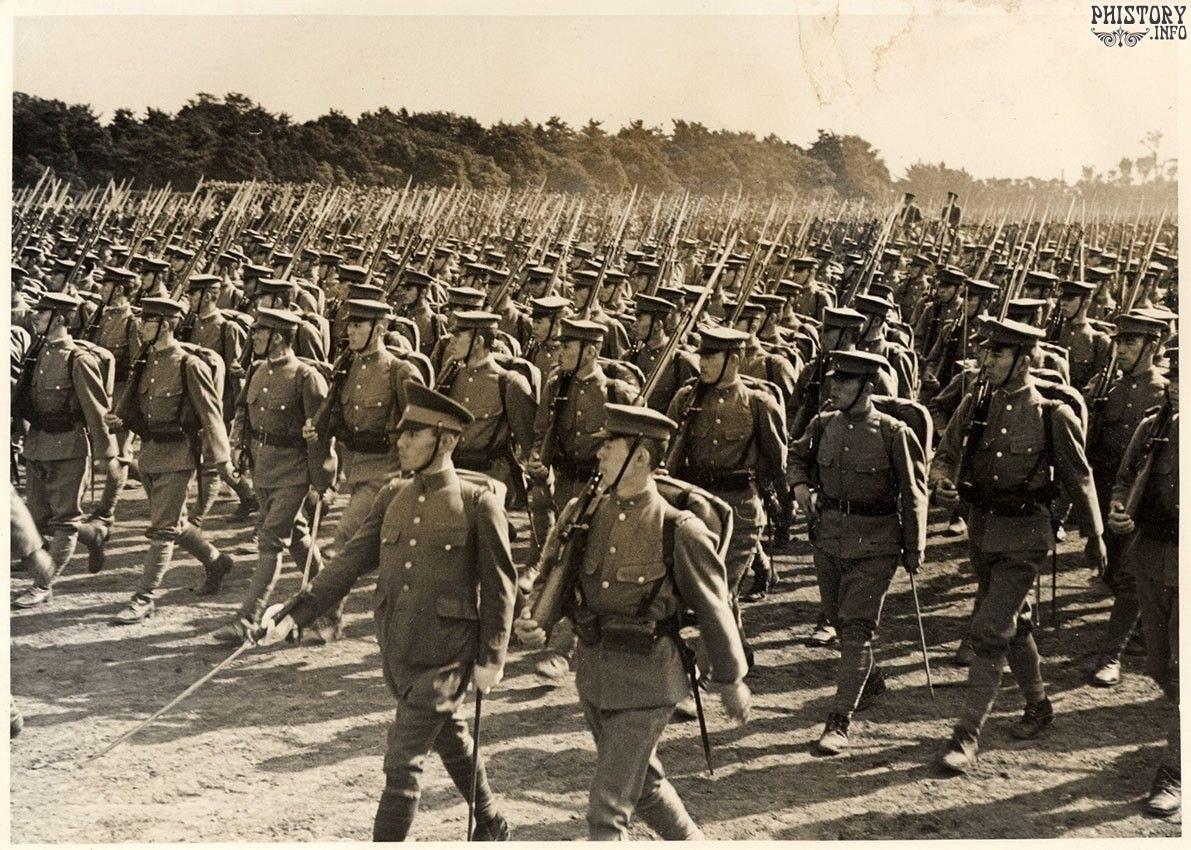
\includegraphics[scale=0.4]{Glava1/_4PjKKM4HkA.jpg}
	%	\label{fig:scipion} % Unique label used for referencing the figure in-text\end{document}
	%	%\addcontentsline{toc}{figure}{Figure \ref{fig:placeholder}} % Uncomment to add the figure to the table of contents%----------------------------------------------------------------------------------------
	\caption{Парад японской армии в Токио, 1921 год}%	CHAPTER 2
\end{figure}

Помимо вышеперечисленного, ещё один очень важный фактор – это так называемые Дзайбацу. Вообще дословно с японского это переводится просто как собственность. Но в приложении к истории Японии от конца XIX века и до Второй мировой речь идёт о глобальных объединениях-монополиях, которые с одной стороны по преимуществу контролировали какую-то часть рынка, а с другой стороны имели дочерние и вспомогательные структуры в самых разных отраслях, которые суммарно обеспечивали такому монстру почти полную автономию. Дзайбацу – отличительная черта развития капитализма в Японии, где стадия хаотической свободной конкуренции и первоначального накопления была преодолена очень быстро, чтобы в итоге породить одну из самых высоких в мире степеней концентрации капитала.

Причём, несмотря на это, он был слабоакционированным. У гигантских трестов и синдикатов были вполне конкретные собственники (откуда и название). Уже этот факт сильно облегчал контакт власти и бизнеса, особенно при обсуждении крупных вопросов, или достижении договорённостей на длительную перспективу. Наёмный управляющий далеко не всегда рискнёт активно вести игру с правительством и брать на себя обязательства. Переговоры с акционерами – всегда сложнейший торг, в котором нужно учитывать массу отдельных личных интересов, а общая консолидированная позиция далеко не всегда достижима. В случае с дзайбацу был тот конкретный человек, с которым можно было переговорить и достигнуть ясного и надёжного соглашения.
Речь, правда, все же идёт не столько о личностях, сколько о кланах – известные параллели тут можно найти с европейскими финансовыми кланами, например знаменитыми Ротшильдами. Но есть и существенная разница. Фактически около дюжины семейств контролировали почти всю национальную экономику. Исходя из этого, они должны были иметь (и имели) колоссальное влияние и силу. Вот только их богатство было практически полностью сконцентрировано в пределах национальных границ. Если те же Ротшильды достаточно быстро стали интернациональной силой, которая, исходя из своей выгоды, делала ставку и избирала в качестве основной своей базы то одно, то другое государство, то судьба кланов-дзайбацу была плотно привязана к Японии. Прежде всего, дело тут было в том, что из Страны Восходящего солнца почти не было экспорта капитала. Источник богатства таких объединений, как Мицубиси или Сумитомо, лежал не в вывозе сырья, или в финансовых спекуляциях, что способствует накоплению свободных, легко перебрасываемых средств, но в промышленности. Капитаны индустрии обладали огромными ресурсами, но они практически полностью находились в деле и не могли быть извлечены из него без фатальных последствий. Для своего функционирования промышленность Японии нуждалась в постоянных закупках сырья, а потому всякая крупная прибыль не выводилась из страны, но обращалась на дальнейшее развитие производства. Всё это придало дзайбацу по необходимости ярко выраженную национальную ориентацию. И заставило искать путей для компромисса и взаимопонимания с высшей политической власти вместо жесткого давления на неё.

Фактически Японии чрезвычайно “повезло” в том отношении, что вместо обыкновенной олигархии сложилась весьма специфическая форма отношений между правительством и крупным бизнесом. Свою роль, конечно, сыграло и сохранение сильной императорской власти с многочисленными прерогативами. Даже император едва ли смог бы перебороть кланы-дзайбацу, если бы они выступили против него разом по какому-либо вопросу. Вот только в реальности для такого рода демаршей не было повода. В то же время, император обладал достаточными рычагами влияния для того, чтобы ослаблять менее лояльные и вознаграждать более лояльные кланы (самый очевидный инструмент – доступ к государственному заказу на военные и инфраструктурные проекты). При этом важно помнить, что ввиду особенностей японского менталитета и общественной структуры монарх был практически гарантированно застрахован от глобального покушения на свою власть. Практически все кланы-дзайбацу имели мелкое самурайское происхождение – со всем вытекающим комплексом представлений о мире, о себе и о своём долге по отношению к государству и Микадо.

На итог сложилась очень выигрышная и сильно поспособствовавшая экономическому росту Японии система, при которой власть хорошо знала и учитывала интересы крупного бизнеса, а он в свою очередь был не только отстранённо лоялен, но деятельно способствовал реализации тех или иных социальных, экономических и внешнеполитических проектов правительства. Вообще такого рода порядок оказался настолько эффективным, что пережил даже поражение в войне, крушение старой Японии и американскую оккупацию. Администрация Макартура приняла ряд приказов, согласно которым 10 основных дзайбацу должны были быть разделены и ликвидированы уже к 1946 году. Действовали во многом по аналогии с имевшим место во времена оные насильственным разделением Стандард Ойл в самой Америке. Результат был схожий – насильственно порванные связи достаточно быстро восстанавливались, формально отдельные компании координировали свои действия на рынке, да и вообще всё было похоже на противника Шварцнеггера из второго Терминатора – разбитый и расколотый он достаточно быстро стекался и собирался воедино заново. Только в Японии всё вышло ещё более провально, чем в США – прежде всего ввиду явно выраженного и всеобщего недовольства не только самих бизнесменов, но и бюрократии и даже работников предприятий – так дзайбацу Мацусита, поначалу должна была быть также закрыта, но была спасена петицией, организованной союзом, в который входили 15 000 рабочих компании и их семьи. В 1950-х термин дзайбацу ушёл в прошлое, уступив место термину кайрецу, которые и посейчас играют ведущую роль в экономике страны, причём большая их часть ведёт более или менее ярко выраженную преемственность по отношению к предшественникам. Мицубиси и Мицуи, Сумитомо и Токай – все они существуют и поныне и руководят огромными империями, включающими в себя самые знаменитые мировые бренды. И по-прежнему плотно взаимодействуют с властью. 

\begin{figure}[h!tb] 
	\centering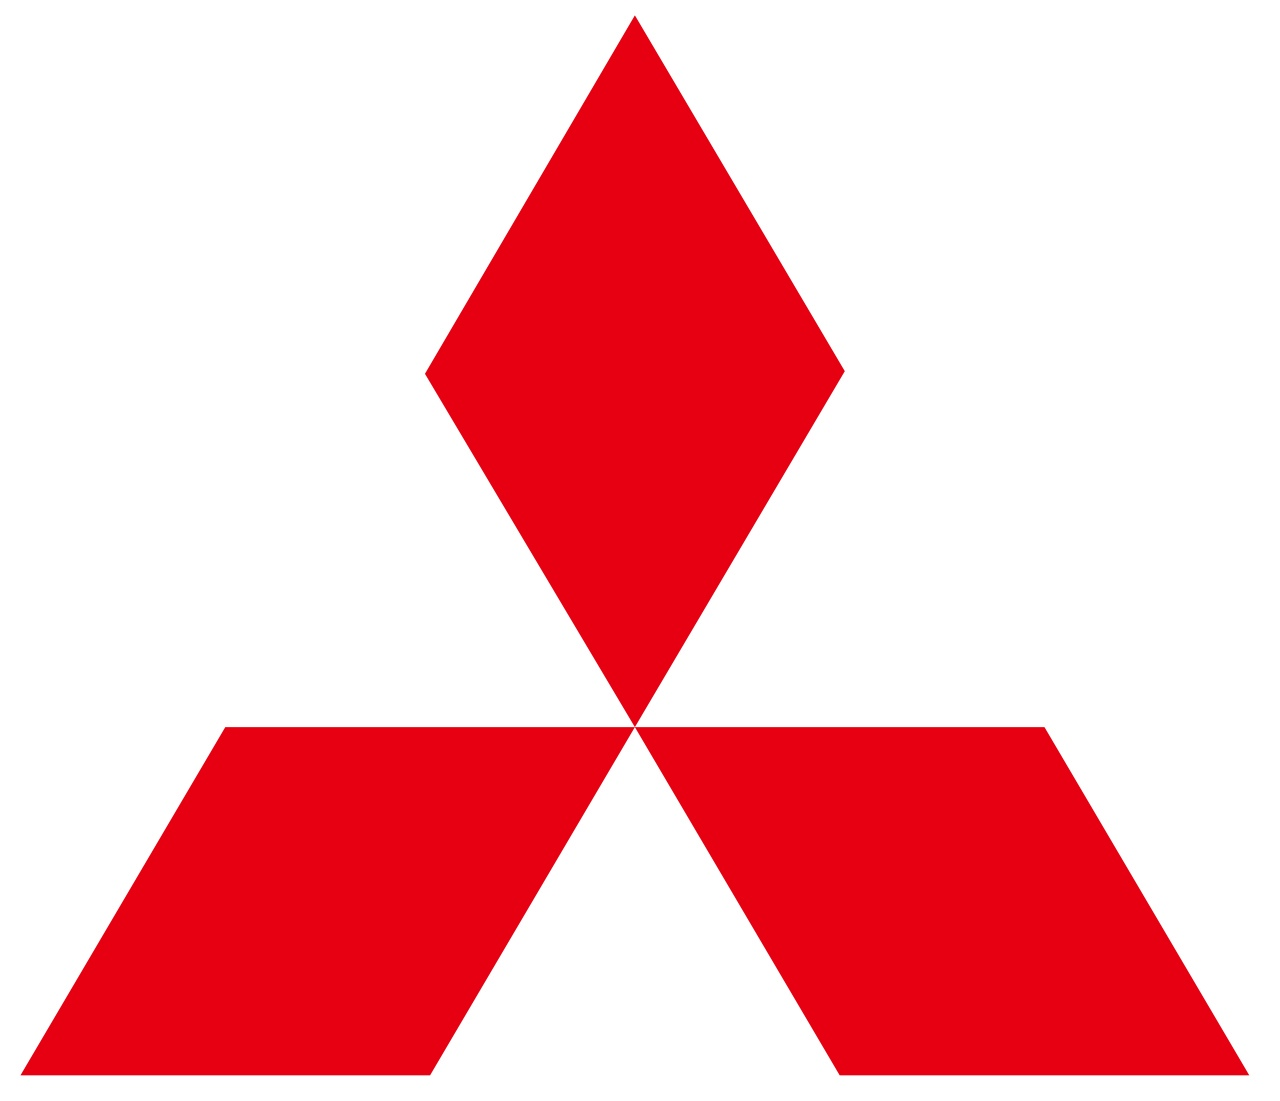
\includegraphics[scale=0.4]{Glava1/xVqA_r2Y8Bs.jpg}
	%	\label{fig:scipion} % Unique label used for referencing the figure in-text\end{document}
	%	%\addcontentsline{toc}{figure}{Figure \ref{fig:placeholder}} % Uncomment to add the figure to the table of contents%----------------------------------------------------------------------------------------
	\caption{Символ дзайбацу Мицубиси, возникшей ещё в 1870-х, и сейчас известен всему миру}%	CHAPTER 2
\end{figure}

Однако вернёмся в предвоенные времена. Как всякий крупный капитал, дзайбацу стремились к расширению – и не могли не сознавать, что собственная ресурсная база их страны не позволяет им достигнуть таких масштабов и оборотов, каких достигли ведущие объединения США, Великобритании, Франции – основных конкурентов японцев в бассейне Тихого океана и в Китае в 1920-е и 1930-е. Вообще идея экспансии должна была представляться главам дзайбацу очень естественной и заманчивой. Так же естественно и то, что в этом отношении они нашли полное понимание со стороны властей. Принципиально другое – экспансия, её плоды для дзайбацу была внесена в негласный договор между ними и правительством. В этом смысле нельзя сказать, что, скажем, решение о развязывании войны с Китаем было прямо продиктовано кланами-дзайбацу, но у руководства Японии было очень чёткое понимание, что даже временный отказ от экспансии может фатально нарушить так удачно отстроенную его симфонию с бизнесом и вообще сделаться началом крупных неприятностей и потрясений. Одним словом, не то чтобы дзайбацу держали империю за горло мертвой хваткой, но не учитывать их интересы было совершенно невозможно.

Итак, ещё раз – экспансия – безусловная необходимость. По этому поводу в Японии имеется общественный консенсус, всеобщая убеждённость. По-своему она даже превосходит убеждённость в необходимости натиска на Восток среди немцев. Японские солдаты и, особенно, офицеры во Вторую мировую будут очень чётко сознавать, что воюют за жизнь и будущее империи. Нам остаётся теперь понять главное, то, что и было вынесено в заглавие серии – какими принципами руководствовалось правительство Страны Восходящего солнца, когда делало шаги в том или ином направлении, и что в итоге привело к столкновению с США, ставшему фатальным для Японии. 

\url{https://vk.com/wall-162479647_82858}